\documentclass[12pt,a4paper]{article}
%%%%%%%%%%%%%%%%%%%%%%%%%%%%%%%%%%%%%%%%%%%%
%                 PACKAGES
%%%%%%%%%%%%%%%%%%%%%%%%%%%%%%%%%%%%%%%%%%%%

% LANGUAGE AND ENCODING
\usepackage[utf8]{inputenc}      % Direct UTF-8 character input
\usepackage[english]{babel}      % Language-specific hyphenation
\usepackage{xstring}

% CORE MATHEMATICS
\usepackage{amsmath}             % AMS math environments (align, gather, etc.)
\usepackage{amssymb}             % AMS math symbols
\usepackage{amsthm}              % Theorem environments
\usepackage{amsfonts}            % AMS fonts
\usepackage{mathtools}           % Extensions to amsmath
\usepackage{esint}               % Extended integral symbols
\usepackage{cancel}              % Diagonal cancellation in math
\usepackage{tcolorbox}           % Good boxes
\tcbuselibrary{most}

\usepackage{lmodern}
\usepackage{bm}                  % Bold math symbols (Greek, etc.)
\usepackage{mathrsfs}            % Ralph Smith's script font
\usepackage{tensor}              % Tensor index notation

% UNITS AND QUANTITIES
\usepackage{siunitx}             % Professional number and unit formatting
\NewCommandCopy\uqty\qty         % Save siunitx's \qty as \uqty
\usepackage{silence}
\WarningFilter{siunitx}{Detected the "physics" package}
\ExplSyntaxOn
\msg_redirect_name:nnn { siunitx } { physics-pkg } { none }
\ExplSyntaxOff

% TABLES AND BOXES
\usepackage{tabulary}            % Tables with automatic width adjustment
\usepackage{mdframed}            % Framed boxes with backgrounds
% \usepackage{chemformula}       % Alternative chemistry notation (commented)

% MATH TOOLS
\usepackage{centernot}           % Centered negation symbol
\usepackage{dcolumn}             % Decimal alignment in tables
\usepackage[shortlabels]{enumitem} % Customizable lists

% GRAPHICS AND FIGURES
\usepackage{graphicx}            % Include images
\usepackage{float}               % Force figure placement with [H]
\usepackage{tikz}                % Powerful diagram drawing
\usetikzlibrary{positioning,arrows,trees,3d,angles} % TikZ libraries
\usepackage{pgfplots}            % Scientific plots based on tikz
\pgfplotsset{compat=1.18}        % PGFPlots compatibility mode
\usepackage{subcaption}          % Subfigures (a), (b), etc.
\usepackage{caption}             % Customize caption formatting
\usepackage{booktabs}            % Professional tables with \toprule

% MULTI-COLUMN AND ARRAYS
\usepackage{multicol}            % Multi-column text layout
\usepackage{array}               % Enhanced table column types

% CHEMISTRY
\usepackage{chemfig}             % Draw molecular structures
\usepackage[version=4]{mhchem}   % Chemical equations in text (\ce{H2O})

% CIRCUITS
\usepackage{circuitikz}          % Circuit diagrams with tikz

% TEXT FORMATTING
\usepackage{blindtext}           % Lorem ipsum placeholder text
\usepackage{titlesec}            % Customize section headings
\usepackage{fancyhdr}            % Custom headers and footers
\usepackage{csquotes}            % Context-sensitive quotes

% HYPERLINKS
\usepackage[colorlinks=true, allcolors=blue]{hyperref} % Clickable links

% PAGE GEOMETRY
\usepackage[top=1.0in,bottom=1.0in,left=1.0in,right=1.0in,marginparwidth=1.75cm]{geometry}

% CODE LISTINGS
\usepackage{xcolor}              % Color definitions
\usepackage{listings}            % Code syntax highlighting
\usepackage{xparse}              % Robust command definitions
\usepackage{braket}              % Dirac bra-ket notation

% PHYSICS PACKAGES (LOADED LAST)
\usepackage[italicdiff]{physics} % Original physics package (d in italics)
\usepackage{physics2}            % Modern physics package
\usephysicsmodule{ab}            % Auto-braces module
\usephysicsmodule{ab.legacy}     % Legacy \abs, \norm, \eval
\usephysicsmodule{nabla.legacy}  % \grad, \div, \curl operators
% \usephysicsmodule{op.legacy}     % Operators like \tr, \Re, \Im
% \usephysicsmodule{diagmat, xmat} % Diagonal and special matrices
% \usephysicsmodule{braket, ab.braket} % Dirac notation
\let\lpc\laplacian               % Alias for Laplacian

%%%%%%%%%%%%%%%%%%%%%%%%%%%%%%%%%%%%%%%%%%%%
%             NEW COMMANDS
%%%%%%%%%%%%%%%%%%%%%%%%%%%%%%%%%%%%%%%%%%%%

%%% MATH OPERATORS
\DeclareMathOperator{\sinc}{sinc}
\DeclareMathOperator{\sgn}{sgn}

%%% INVERSE TRIGONOMETRIC OPERATORS
\renewcommand{\asin}{\sin^{-1}}
\renewcommand{\acos}{\cos^{-1}}
\renewcommand{\atan}{\tan^{-1}}
\renewcommand{\acsc}{\csc^{-1}}
\renewcommand{\asec}{\sec^{-1}}
\renewcommand{\acot}{\cot^{-1}}

\newcommand{\asinh}{\sinh^{-1}}
\newcommand{\acosh}{\cosh^{-1}}
\newcommand{\atanh}{\tanh^{-1}}
\newcommand{\acsch}{\csch^{-1}}
\newcommand{\asech}{\sech^{-1}}
\newcommand{\acoth}{\coth^{-1}}
% \DeclareMathOperator{\arcsin}{arcsin}
% \DeclareMathOperator{\arccos}{arccos}
% \DeclareMathOperator{\arctan}{arctan}
% \DeclareMathOperator{\arccsc}{arccsc}
% \DeclareMathOperator{\arcsec}{arcsec}
% \DeclareMathOperator{\arccot}{arccot}
\DeclareMathOperator{\arsinh}{arsinh}
\DeclareMathOperator{\arcosh}{arcosh}
\DeclareMathOperator{\artanh}{artanh}
\DeclareMathOperator{\arcsch}{arcsch}
\DeclareMathOperator{\arsech}{arsech}
\DeclareMathOperator{\arcoth}{arcoth}

%%% NUMBER SETS
\newcommand{\R}{\mathbb{R}}          % Real numbers
\newcommand{\Z}{\mathbb{Z}}          % Integers
\newcommand{\Q}{\mathbb{Q}}          % Rational numbers
\newcommand{\C}{\mathbb{C}}          % Complex numbers
\newcommand{\N}{\mathbb{N}}          % Natural numbers
\newcommand{\K}{\mathbb{K}}          % Field R or C
\newcommand{\bb}[1]{\mathbb{#1}}     % Generic blackboard bold

%%% PARTIAL DIFFERENTIALS
\newcommand{\p}{\partial}            % Partial symbol

%%% VECTOR CALCULUS
\newcommand{\krondelta}[1]{\delta_{#1}}
\newcommand{\levicivita}[1]{\varepsilon_{#1}}
\newcommand{\ihat}{\vu*{\imath}}
\newcommand{\jhat}{\vu*{\jmath}}
\newcommand{\khat}{\vu*{k}}
\newcommand{\rhohat}{\vu*{\rho}}
\newcommand{\phihat}{\vu*{\phi}}
\newcommand{\thetahat}{\vu*{\theta}}
\newcommand{\rhat}{\vu*{r}}
\newcommand{\inv}{^{-1}}
\newcommand{\vell}{\boldsymbol{\ell}}

%%% DIFFERENTIALS AND TRANSFORMS
\newcommand{\laplace}[1]{\mathscr{L}\qty{#1}}
\newcommand{\invlaplace}[1]{\mathscr{L}^{-1}\qty{#1}}
\newcommand{\unitstep}[1]{\mathscr{U}\qty{#1}}
\newcommand{\intfty}{\int_{-\infty}^{+\infty}}

%%% PARENTHESES
\newcommand{\floor}[1]{\lfloor #1 \rfloor}
\newcommand{\ceiling}[1]{\lceil #1 \rceil}
\newcommand{\round}[1]{\lfloor #1 \rceil}
\newcommand{\nvec}[3]{\left\langle #1 , #2 , #3 \right\rangle}
\newcommand{\tline}[1]{\hrule \vspace{#1} \hrule}
\newcommand{\blank}[1]{\hspace*{#1}}

%%% TRANSFORM OPERATORS
\newcommand{\Laplace}{\mathscr{L}}
\newcommand{\Fourier}{\mathscr{F}}

%%% LOGICAL OPERATORS
\newcommand{\union}{\cup}
\newcommand{\intersect}{\cap}
\newcommand{\defined}{:=}

%%% COMPLEX ANALYSIS
\newcommand{\Arg}{\operatorname{Arg}}
\newcommand{\Hol}{\operatorname{Hol}}
\newcommand{\Log}{\operatorname{Log}}

%%% LINEAR ALGEBRA
\newcommand{\Span}[1]{\operatorname{span}\qty(#1)}
\newcommand{\Rank}[1]{\operatorname{rank}\qty(#1)}
\newcommand{\nullity}[1]{\operatorname{nullity}\qty(#1)}
\DeclareMathOperator{\image}{im}

%%% TOPOLOGY
\newcommand{\Id}{\operatorname{Id}}
\newcommand{\Image}[1]{\operatorname{Im}\qty(#1)}
\newcommand{\comp}{^{c}}
\newcommand{\Prob}[1]{\operatorname{Pr}\qty(#1)}
\newcommand{\du}{\mathrm{d}}
\newcommand{\topo}[1]{\mathcal{#1}}

%%% MISCELLANEOUS
\newcommand{\notimplies}{\centernot\implies}

\NewDocumentCommand{\dimu}{O{\mkern-3mu} m}{
\left[
#1
\left[#2\right]
#1
\right]
}

\newcommand{\id}{\operatorname{id}}
\newcommand{\contradiction}{\Rightarrow\!\Leftarrow}
\newcommand{\transition}[3]{{_{#2}\mathbf{#1}_{#3}}}
\newcommand{\barline}{\vspace{10pt}\hrule\vspace{10pt}}
\newcommand{\eqques}{\stackrel{?}{=}}
\newcommand{\Gammaf}[1]{\Gamma\qty(#1)}
\renewcommand\qedsymbol{$\square$}


%%%%%%%%%%%%%%%%%%%%%%%%%%%%%%%%%%%%%%%%%%%%
%       CUSTOM HEADER / SECTION STYLES
%%%%%%%%%%%%%%%%%%%%%%%%%%%%%%%%%%%%%%%%%%%%

\fancypagestyle{titleheader}{
  \fancyhead{}
  \fancyhead{\vspace{2cm}\tline{3pt}\fancyfoot[c]{\thepage}}
  \renewcommand{\headrulewidth}{0pt}
}
\newcommand{\titlebars}{
  \maketitle
  \tline{3pt}
  \thispagestyle{titleheader}
}

%%% CUSTOM SUBSUBSUBSECTION (4-LEVEL HEADINGS)
\titleclass{\subsubsubsection}{straight}[\subsection]
\newcounter{subsubsubsection}[subsubsection]
\renewcommand\thesubsubsubsection{\thesubsubsection.\arabic{subsubsubsection}}
\renewcommand\theparagraph{\thesubsubsubsection.\arabic{paragraph}}
\titleformat{\subsubsubsection}{\normalfont\normalsize\bfseries}{\thesubsubsubsection}{1em}{}
\titlespacing*{\subsubsubsection}{0pt}{3.25ex plus 1ex minus .2ex}{1.5ex plus .2ex}

\makeatletter
\renewcommand\paragraph{\@startsection{paragraph}{5}{\z@}{3.25ex \@plus1ex \@minus.2ex}{-1em}{\normalfont\normalsize\bfseries}}
\renewcommand\subparagraph{\@startsection{subparagraph}{6}{\parindent}{3.25ex \@plus1ex \@minus .2ex}{-1em}{\normalfont\normalsize\bfseries}}
\def\toclevel@subsubsubsection{4}
\def\toclevel@paragraph{5}
\def\toclevel@subparagraph{6}
\def\l@subsubsubsection{\@dottedtocline{4}{7em}{4em}}
\def\l@paragraph{\@dottedtocline{5}{10em}{5em}}
\def\l@subparagraph{\@dottedtocline{6}{14em}{6em}}
\makeatother
\setcounter{secnumdepth}{4}
\setcounter{tocdepth}{4}

%%% CUSTOM SECTION TITLE FONT SIZES
% \titleformat*{\section}{\LARGE\bfseries}
% \titleformat*{\subsection}{\Large\bfseries}
% \titleformat*{\subsubsection}{\large\bfseries}
% \setlength{\parskip}{10pt}

%%%%%%%%%%%%%%%%%%%%%%%%%%%%%%%%%%%%%%%%%%%%
%             ENVIRONMENTS
%%%%%%%%%%%%%%%%%%%%%%%%%%%%%%%%%%%%%%%%%%%%

\newenvironment{amatrix}[1]{%
  \left(
  \begin{array}{@{}*{#1}{c}|c@{}}}{
\end{array}\right)}

\newenvironment{abmatrix}[1]{%
  \left[
  \begin{array}{@{}*{#1}{c}|c@{}}}{
\end{array}\right]}


%%%%%%%%%%%%%%%%%%%%%%%%%%%%%%%%%%%%%%%%%%%%
%          THEOREM STYLES
%%%%%%%%%%%%%%%%%%%%%%%%%%%%%%%%%%%%%%%%%%%%

% \theoremstyle{definition}
% \newtheorem{theorem}{Theorem}[subsection]
% \newtheorem{corollary}{Corollary}[theorem]
% \newtheorem{lemma}[theorem]{Lemma}
% \newtheorem{definition}{Definition}[subsection]
% \newtheorem{example}{Example}[subsection]

% \theoremstyle{remark}
% \newtheorem*{remark}{Remark}
% \newtheorem*{solution}{Solution}
% \newtheorem*{note}{Note}

%%%%%%%%%%%%%%%%%%%%%%%%%%%%%%%%%%%%%%%%%%%%
%        CODE LISTING STYLE
%%%%%%%%%%%%%%%%%%%%%%%%%%%%%%%%%%%%%%%%%%%%


% ============================================
% PYTHON STYLE
% ============================================
\definecolor{vscodeBackground}{RGB}{255,255,255}
\definecolor{vscodeForeground}{RGB}{10,10,10}
\definecolor{vscodeKeyword}{RGB}{60,60,200}
\definecolor{vscodeString}{RGB}{230,0,0}
\definecolor{vscodeComment}{RGB}{0,100,0}
\definecolor{vscodeFunction}{RGB}{220,220,170}
\definecolor{vscodeOperator}{RGB}{212,212,212}
\definecolor{vscodeNumber}{RGB}{181,206,168}

\lstdefinestyle{vscodepython}{
    backgroundcolor=\color{vscodeBackground},
    basicstyle=\ttfamily\footnotesize\color{vscodeForeground},
    commentstyle=\color{vscodeComment},
    keywordstyle=\color{vscodeKeyword}\bfseries,
    stringstyle=\color{vscodeString},
    numberstyle=\tiny\color{vscodeForeground},
    identifierstyle=\color{vscodeForeground},
    morekeywords={True, False, None, and, as, assert, async, await, break, class,
        continue, def, del, elif, else, except, finally, for, from, global, if,
        import, in, is, lambda, nonlocal, not, or, pass, raise, return, try,
        while, with, yield},
    frame=single,
    rulecolor=\color{vscodeForeground},
    breaklines=true,
    numbers=left,
    numbersep=5pt,
    showstringspaces=false,
    tabsize=4,
    captionpos=b,
}

% ============================================
% C/C++ STYLE (FIXED)
% ============================================
\definecolor{vscodeType}{RGB}{0,150,200}
\definecolor{vscodePreprocessor}{RGB}{150,0,150}
\definecolor{vscodeFunction}{RGB}{180,100,0}
\definecolor{vscodeOperator}{RGB}{180,60,180}

\lstdefinestyle{vscodecpp}{
    backgroundcolor=\color{vscodeBackground},
    basicstyle=\ttfamily\scriptsize\color{vscodeForeground},
    commentstyle=\color{vscodeComment},
    stringstyle=\color{vscodeString},
    numberstyle=\tiny\color{vscodeForeground},
    identifierstyle=\color{vscodeForeground},
    %
    % Keywords (class 1)
    keywords={auto, break, case, catch, class, const, constexpr, continue,
        default, delete, do, else, enum, explicit, extern, false, final,
        for, friend, goto, if, inline, mutable, namespace, new, noexcept,
        nullptr, operator, override, private, protected, public, register,
        return, sizeof, static, static_assert, struct, switch, template,
        this, throw, true, try, typedef, typeid, typename, using, virtual,
        volatile, while},
    %
    % Types (class 2) – highlighted with emph
    emph={bool, char, char16_t, char32_t, double, float, int, long, short,
          signed, unsigned, void, wchar_t, size_t, ptrdiff_t},
    emphstyle={\color{vscodeType}\bfseries},
    %
    % Preprocessor (class 3)
    emph={[2]define, elif, else, endif, error, if, ifdef, ifndef, include,
          line, pragma, undef},
    emphstyle={[2]\color{vscodePreprocessor}\bfseries},
    %
    % Standard library functions (class 4)
    emph={[3]printf, scanf, fprintf, fscanf, sprintf, sscanf, getchar, putchar,
          gets, puts, fopen, fclose, fread, fwrite, malloc, calloc, realloc,
          free, exit, abort, assert, system, getenv, qsort, bsearch, memcpy,
          memset, memcmp, strlen, strcpy, strncpy, strcat, strncat, strcmp,
          strncmp, strstr, strtok, atoi, atof, atol, rand, srand, time, clock,
          pow, sqrt, exp, log, log10, sin, cos, tan, asin, acos, atan, atan2,
          fabs, floor, ceil, fmod, feof, ferror, clearerr, remove, rename,
          tmpfile, tmpnam, setbuf, setvbuf, rewind, fgetc, fputc, ungetc,
          fgets, fputs},
    emphstyle={[3]\color{vscodeFunction}\bfseries},
    %
    % C++ extra keywords (add to class 1)
    morekeywords={alignas, alignof, and, and_eq, bitand, bitor, compl,
        concept, const_cast, decltype, dynamic_cast, module, not, not_eq,
        or, or_eq, reinterpret_cast, requires, static_cast, xor, xor_eq},
    %
    % STL types and functions (add to class 4 via emph again)
    emph={[4]std, vector, map, set, string, array, deque, list, queue, stack,
          pair, tuple, unique_ptr, shared_ptr, weak_ptr, make_shared, make_unique,
          move, forward, function, bind, cout, cin, endl, cerr, clog,
          ifstream, ofstream, fstream, stringstream, istringstream, ostringstream,
          sort, find, transform, accumulate, for_each, copy, reverse, unique,
          remove, replace, swap, min, max, lower_bound, upper_bound, binary_search},
    emphstyle={[4]\color{vscodeFunction}\bfseries},
    %
    frame=single,
    rulecolor=\color{vscodeForeground},
    breaklines=true,
    numbers=left,
    numbersep=5pt,
    showstringspaces=false,
    tabsize=4,
    captionpos=b,
}

% ============================================
% SET DEFAULTS
% ============================================
\lstset{style=vscodepython, language=Python}


%% EMPHASIS BOX

\newtcolorbox{emphasis}{
  colback=white,        % White background
  colframe=black,       % Black border
  boxrule=0.5pt,        % Border thickness
  arc=0pt,              % Sharp corners (0pt = no rounding)
  left=6pt,             % Left padding
  right=6pt,            % Right padding
  top=6pt,              % Top padding
  bottom=6pt,           % Bottom padding
  boxsep=0pt,           % No extra separation
  before upper={
    \setlength{\abovedisplayskip}{0pt}
    \setlength{\abovedisplayshortskip}{0pt}
    \setlength{\belowdisplayskip}{0pt}
    \setlength{\belowdisplayshortskip}{0pt}
  }
}

%%%%%%%%%%%%%%%%%%%%%%%%%%%%%%%%%%%%%%%%%%%%
%             DOCUMENT SETTINGS
%%%%%%%%%%%%%%%%%%%%%%%%%%%%%%%%%%%%%%%%%%%%

\setlength{\parindent}{2em}
\setlength{\parskip}{5pt}
\newlength{\originalparindent}
\newlength{\originalparskip}
\AtBeginDocument{%
    \setlength{\originalparindent}{\parindent}%
    \setlength{\originalparskip}{\parskip}%
}
\numberwithin{equation}{section}

% SECTION TITLE FONT SIZES (move here from preset)
\titleformat*{\section}{\LARGE\bfseries}
\titleformat*{\subsection}{\Large\bfseries}
\titleformat*{\subsubsection}{\large\bfseries}
\titleformat*{\subsubsubsection}{\large\bfseries}

% CUSTOM SECTION COMMANDS
\newcommand{\module}[1]{%
    \clearpage
    \refstepcounter{section}
    \vspace*{1cm}
    {\LARGE\bfseries\noindent Module \thesection\par}
    \vspace{0.5cm}
    {\noindent\Huge\bfseries #1\par}
    \vspace{2cm}
    \addcontentsline{toc}{section}{Module \thesection : #1}
}

\newcommand{\unitsec}[1]{%
    \clearpage
    \refstepcounter{section}
    \vspace*{1cm}
    {\LARGE\bfseries\noindent Unit \thesection\par}
    \vspace{0.5cm}
    {\noindent\huge\bfseries #1\par}
    \vspace{1.5cm}
    \addcontentsline{toc}{section}{Unit \thesection : #1}
}

\newcommand{\chaptersec}[2][\relax]{%
    \clearpage
    \refstepcounter{section}
    \vspace*{0.5cm}
    {\LARGE\bfseries\noindent Chapter \thesection\par}
    \vspace{0.5cm}
    {\noindent\huge\bfseries
        \ifx\relax#1\relax
            #2%
        \else
            #1%
        \fi
        \par
    }
    \vspace{1.5cm}
    \addcontentsline{toc}{section}{Chapter \thesection : #2}
}

%%% PROBLEM ENVIRONMENT (was in preset.tex, now here)
\newenvironment{problem}{%
    \hrule
    \vspace{5pt}
}{%
    \vspace{10pt}\hrule\vspace{10pt}
}

\newenvironment{solution_pset}{%
    \noindent\textbf{\Large Solution}\\[0.5cm]
}{%
    \newpage
}


%%% DEFINITION ENVIRONMENT
% Definition counter linked to section
\newcounter{definition}[section]
\renewcommand{\thedefinition}{\thesection.\arabic{definition}}

\newtcolorbox{definition}[2][]{%
    colback=white,
    colframe=black,
    boxrule=0.5pt,
    arc=0pt,
    left=6pt,
    right=6pt,
    top=6pt,
    bottom=6pt,
    fonttitle=\bfseries,
    title={%
        \stepcounter{definition}% Increment counter
        Definition \thedefinition{} : #2% Then display
    },
    #1
}

%%% EXAMPLE ENVIRONMENT
% Example counter linked to section
\newcounter{example}[section]
\renewcommand{\theexample}{\thesection.\arabic{example}}

\newtcolorbox{example}[2][]{%
    breakable,
    colback=white,
    colframe=blue,
    boxrule=0.5pt,
    arc=4pt,
    left=6pt,
    right=6pt,
    top=6pt,
    bottom=6pt,
    fonttitle=\bfseries,
    parbox=false,  % Don't use parbox mode
    before upper={%
        \setlength{\parindent}{\originalparindent}%
        \setlength{\parskip}{\originalparskip}%
        \noindent%
    },
    title={%
        \refstepcounter{example}%
        Example \theexample{} : #2%
    },
    #1
}

%%% THEOREM ENVIRONMENT
% Theorem counter linked to section
\newcounter{theorem}[section]
\renewcommand{\thetheorem}{\thesection.\arabic{theorem}}
\definecolor{darkred}{RGB}{139, 0, 0} 
\newenvironment{theorem}[2][]{%
    \refstepcounter{theorem}%
    \begin{tcolorbox}[
        colback=white,
        colframe=darkred,
        coltitle=white,
        colbacktitle=darkred,
        boxrule=0.5pt,
        arc=0pt,
        left=6pt,
        right=6pt,
        top=6pt,
        bottom=6pt,
        fonttitle=\bfseries,
        title={Theorem \thetheorem{} : #2},
        #1
    ]
}{%
    \end{tcolorbox}%
}

%%% NOTE ENVIRONMENT
\definecolor{darkgray}{RGB}{100, 100, 100}

\newtcolorbox{note}{%
    colback=white,
    colframe=darkgray,
    boxrule=0.5pt,
    arc=0pt,
    left=6pt,
    right=6pt,
    top=6pt,
    bottom=6pt,
    before upper={%
        \noindent{\textit{Note : }}\par\vspace{1em}%
    }
}

%%% REMARK ENVIRONMENT
\newtcolorbox{remark}{%
    colback=white,
    colframe=darkgray,
    boxrule=0.5pt,
    arc=0pt,
    left=6pt,
    right=6pt,
    top=6pt,
    bottom=6pt,
    before upper={%
        \noindent\textbf{\textit{Remark : }}\par\vspace{1em}%
    }
}


\begin{document}
	\begin{titlepage}
    \vspace*{2.5in}
    \hrule
    \vspace{3pt}
    \hrule
    \vspace{0.25in}
    \begin{center}
		{
			\Large 
			\textsc{
				University of the Philippines Diliman
			}
			\\[4pt]
			College of Science
			\\[4pt]
			National Institute of Physics
		}
		\\[0.5cm]
		{
			\Huge
			\textbf{
				Physics 180 THV-1
				\\[5pt]
				Problem Set 6-7
			}
		}
		\\[0.75cm]
		{
			\Large 
			\textsc{
				Vercil Juan
			}
		}\\[5pt] 
		{
			\large 
			IV - BS Physics
		}
    \end{center}
    \vspace{0.25in}
    \hrule
    \vspace{3pt}
    \hrule 
    \vfill
    \begin{center}
    {\large 
		September 4, 2026
	}
    \end{center}
\end{titlepage}

	% ===========================
	% PROBLEM SET 6
	% ===========================
	\stepcounter{section}
	\section*{
		Problem 6.1
	}
	\begin{problem}
		Find the \textbf{second-order} and the \textbf{third-order} terms in the 
		transition matrix element $T_{fi}$ of Fermi's golden rule.
	\end{problem}
	\begin{solution_pset}
		\nocite{flores2026}
		We start from the expansion of the state in terms of the eigenstates
		$\ket{\phi_k}$ of the unperturbed Hamiltonian,
		\begin{equation}
			\ket{\psi(t)}
			=
			\sum_k c_k(t)\ket{\phi_k}e^{-iE_k t}.
			\label{eq:state-expansion}
		\end{equation}

		Substituting (\ref{eq:state-expansion}) into the time-dependent Schr\"odinger
		equation with interaction Hamiltonian $\hat H'$ gives
		\begin{equation}
			i\sum_k \dv{c_k}{t}\ket{\phi_k}e^{-iE_k t}
			=
			\sum_k \hat H' c_k(t)\ket{\phi_k}e^{-iE_k t}.
			\label{eq:coefficient-equation}
		\end{equation}

		Taking the inner product with $\bra{\phi_f}$ gives the differential equation
		for the coefficient $c_f(t)$ corresponding to transitions to the particular
		final state $\ket{f}=\ket{\phi_f}$. Under the first-order approximation used
		in the lecture, $c_i(t)\approx 1$ and $c_{k\neq i}(t)\approx 0$, giving
		\begin{equation}
			\dv{c_f}{t}
			=
			-i\matrixel{f}{\hat H'}{i}
			e^{i(E_f-E_i)t}.
			\label{eq:first-order-cf}
		\end{equation}

		The lecture defines the transition matrix element by
		\begin{equation}
			T_{fi}
			=
			\matrixel{f}{\hat H'}{i}.
			\label{eq:Tfi}
		\end{equation}

		To obtain the higher-order terms, we no longer restrict the sum in
		(\ref{eq:coefficient-equation}) to the initial state. We write the coefficients
		as an expansion in orders of the perturbing Hamiltonian,
		\begin{equation}
			c_f(t)
			=
			c_f^{(0)}(t)
			+
			c_f^{(1)}(t)
			+
			c_f^{(2)}(t)
			+
			c_f^{(3)}(t)
			+\cdots.
			\label{eq:coefficient-expansion}
		\end{equation}

		The zeroth-order coefficients satisfy
		\begin{equation}
			c_i^{(0)}(t)=1,
			\qquad
			c_{k\neq i}^{(0)}(t)=0.
			\label{eq:zeroth-order}
		\end{equation}

		For an intermediate state $\ket{n}$, the first-order coefficient follows
		from the same differential equation as (\ref{eq:first-order-cf}),
		\begin{equation}
			\dv{c_n^{(1)}}{t}
			=
			-i\matrixel{n}{\hat H'}{i}
			e^{i(E_n-E_i)t}.
			\label{eq:first-order-cn}
		\end{equation}

		Integrating (\ref{eq:first-order-cn}) from $0$ to $t$ gives
		\begin{equation}
			\begin{aligned}
			c_n^{(1)}(t)
			&=
			-i\matrixel{n}{\hat H'}{i}
			\int_0^t
			\dd{t'}\,e^{i(E_n-E_i)t'}
			\\
			&=
			-\matrixel{n}{\hat H'}{i}
			\frac{e^{i(E_n-E_i)t}-1}{E_n-E_i}.
			\end{aligned}
			\label{eq:first-order-cn-integrated}
		\end{equation}

		We now substitute (\ref{eq:first-order-cn-integrated}) into the equation for
		$c_f(t)$. The second-order contribution is now therefore
		\begin{equation}
			\dv{c_f^{(2)}}{t}
			=
			-i\sum_n
			\matrixel{f}{\hat H'}{n}
			e^{i(E_f-E_n)t}
			c_n^{(1)}(t).
			\label{eq:second-order-cf}
		\end{equation}

		Using (\ref{eq:first-order-cn-integrated}), we have
		\begin{equation}
			\begin{aligned}
			\dv{c_f^{(2)}}{t}
			&=
			i\sum_n
			\frac{
				\matrixel{f}{\hat H'}{n}
				\matrixel{n}{\hat H'}{i}
			}{
				E_n-E_i
			}
			\left[
				e^{i(E_f-E_i)t}
				-
				e^{i(E_f-E_n)t}
			\right].
			\end{aligned}
			\label{eq:second-order-cf-expanded}
		\end{equation}

		The first term in (\ref{eq:second-order-cf-expanded}) has the same time
		dependence as the first-order result in (\ref{eq:first-order-cf}). This is the
		term that contributes to the transition matrix element for the transition
		from $\ket{i}$ to $\ket{f}$. Thus, comparing with (\ref{eq:first-order-cf}),
		the second-order transition matrix element is
		\begin{equation}
			\boxed{
				T_{fi}^{(2)}
				=
				\sum_n
				\frac{
					\matrixel{f}{\hat H'}{n}
					\matrixel{n}{\hat H'}{i}
				}{
					E_i-E_n
				}
			}
			\label{eq:Tfi-second}
		\end{equation}

		Hence, to second order, the transition proceeds through an intermediate
		state $\ket{n}$,

		\begin{equation}
			\ket{i}
			\rightarrow
			\ket{n}
			\rightarrow
			\ket{f}.
			\label{eq:second-order-transition}
		\end{equation}

		For the third-order term, we repeat the same procedure. The second-order
		coefficient for an intermediate state $\ket{m}$ contains a contribution
		through another intermediate state $\ket{n}$,

		\begin{equation}
			c_m^{(2)}(t)
			\supset
			\sum_n
			\frac{
				\matrixel{m}{\hat H'}{n}
				\matrixel{n}{\hat H'}{i}
			}{
				(E_i-E_m)(E_i-E_n)
			}
			e^{i(E_m-E_i)t}.
		\label{eq:second-order-cm}
		\end{equation}

		Substituting (\ref{eq:second-order-cm}) into the coefficient equation gives
		the contribution to $c_f^{(3)}$ with the same time dependence as the
		first-order transition,

		\begin{equation}
			\begin{aligned}
			\dv{c_f^{(3)}}{t}
			&\supset
			-i
			\sum_{m,n}
			\frac{
				\matrixel{f}{\hat H'}{m}
				\matrixel{m}{\hat H'}{n}
				\matrixel{n}{\hat H'}{i}
			}{
				(E_i-E_m)(E_i-E_n)
			}
			e^{i(E_f-E_i)t}.
			\end{aligned}
			\label{eq:third-order-cf}
		\end{equation}

		Comparing (\ref{eq:third-order-cf}) with the form of the first-order
		differential equation in (\ref{eq:first-order-cf}), the third-order transition
		matrix element is therefore

		\begin{equation}
			\boxed{
				T_{fi}^{(3)}
				=
				\sum_{m,n}
				\frac{
					\matrixel{f}{\hat H'}{m}
					\matrixel{m}{\hat H'}{n}
					\matrixel{n}{\hat H'}{i}
				}{
				(E_i-E_m)(E_i-E_n)
				}
			}
			\label{eq:Tfi-third}
		\end{equation}

		% The corresponding sequence of transitions is

		% \begin{equation}
		% 	\ket{i}
		% 	\rightarrow
		% 	\ket{n}
		% 	\rightarrow
		% 	\ket{m}
		% 	\rightarrow
		% 	\ket{f}.
		% 	\label{eq:third-order-transition}
		% \end{equation}

		Therefore, extending the transition matrix element defined in
		(\ref{eq:Tfi}) to higher orders,
		\begin{equation}
			\begin{aligned}
			T_{fi}
			&=
			T_{fi}^{(1)}
			+
			T_{fi}^{(2)}
			+
			T_{fi}^{(3)}
			+\cdots
			\\
			&=
			\matrixel{f}{\hat H'}{i}
			+
			\sum_n
			\frac{
				\matrixel{f}{\hat H'}{n}
				\matrixel{n}{\hat H'}{i}
			}{
				E_i-E_n
			}
			+
			\sum_{m,n}
			\frac{
				\matrixel{f}{\hat H'}{m}
				\matrixel{m}{\hat H'}{n}
				\matrixel{n}{\hat H'}{i}
			}{
				(E_i-E_m)(E_i-E_n)
			}
			+\cdots.
			\end{aligned}
			\label{eq:Tfi-expansion}
		\end{equation}
	\end{solution_pset}
	\newpage

	% ===========================
	% PROBLEM SET 7
	% ===========================
	\stepcounter{section}
	\section*{
		Problem 7.1
	}
	\begin{problem}
		The semi-major axis $a$ and semi-major axis $b$ of a prolate spheroid
		with eccentricity $x$ are related through
		\begin{equation}
			\label{eq:prolate-relation}
			b = \sqrt{1-x^2}a
		\end{equation}
		If the volume and surface area of the prolate spheroid are
		\begin{equation}
			\label{eq:v-prolate}
			V_\text{prolate}
			=
			\frac{4}{3}\pi ab^2 
		\end{equation}
		\begin{equation}
			\label{eq:s-prolate}
			S_\text{prolate}
		    =
			2\pi b \pqty{
				b + \frac{
					a \sin\inv(x)
				}{x} 
			}
		\end{equation}
		and defining $\displaystyle \varepsilon =\frac{1}{3} x^2$, show that the equations in slide
		36 (reproduced below) hold for small values of $x$.
		\begin{equation}
			\label{eq:a2-term}
			a_2 A^{\frac{2}{3}} \to a_2 A^\frac{2}{3} \pqty{
				1 + \frac{2}{5} \varepsilon^2
			} 
		\end{equation}
		\begin{equation}
			\label{eq:a3-term}
			a_3 \frac{Z^2}{A^\frac{1}{3}} 
			\to
			a_3 \frac{Z^2}{A^\frac{1}{3}} 
			\pqty{
				1 - \frac{1}{5}
				\varepsilon^{2}
			}
		\end{equation}
	\end{problem}
	\begin{solution_pset}
		We tackle the surface and coulomb term separately. A key 
		observation here is that $a$ and $b$ must be adjusted so that the 
		volume of a corresponding sphere remains constaint. The SEMF equations are fundamentally 
		based on the assumption of a spherical nucleus, and as such changes on that assumption
		means the terms scale respectively. 

		Let $R$ be the radius of the sphere
		having the same volume as the spheroid. From (\ref{eq:v-prolate}), we have
		\[
			\frac{4}{3}\pi ab^2 = \frac{4}{3}\pi R^3  
		\]
		
		Using (\ref{eq:prolate-relation}), $b = a\sqrt{1- x^2}$, we have
		\[
			a^3(1-x^2) = R^3
		\]
		and hence,
		\begin{equation}
			\label{eq:a}
			a = 
			R(1-x^2)^{-1/3}
		\end{equation}
		and
		\begin{equation}
			\label{eq:b}
			b = R(1-x^2)^{1/6}
		\end{equation}
		From this, we begin the proof.
		\paragraph{Surface term}
		\begin{proof}
		   For a spherical nucleus, the surface area $S_0$ is
		   \[
				S_0 = 4\pi R^2
		   \]	
		   Substituting (\ref{eq:a}) and (\ref{eq:b}) into (\ref{eq:s-prolate}), we have
		   \begin{align*}
			    S_\text{prolate} 
				&= 
				2\pi 
				R(1-x^2)^{1/6}
				\pqty{
					R(1-x^2)^{1/6}
					+ \frac{
						R(1-x^2)^{-1/3}
						\sin\inv(x)
					}{x} 
				}\\
				&=
				2\pi 
				R^2(1-x^2)^{1/6}
				\pqty{
					(1-x^2)^{1/6}
					+ \frac{
						(1-x^2)^{-1/3}
						\sin\inv(x)
					}{x} 
				}
		   \end{align*}

		   Dividing by $S_0$, we find
		   \begin{equation}
		   	\label{eq:SprolateS0}
			   \frac{
					S_\text{prolate} 
				}{
					S_0
				} 
				=
				\frac{1}{2} 
				(1-x^2)^{1/6}
				\pqty{
					(1-x^2)^{1/6}
					+ \frac{
						(1-x^2)^{-1/3}
						\sin\inv(x)
					}{x} 
				}
		   \end{equation}

		   For small $x$, i.e., $x\ll 1$, the following terms can be expanded as\footnote{Trivial to show, taylor series.}
		   \begin{align*}
			   \frac{
				   \sin\inv(x)
			   }{
				   x
			   } 
			   &= 
			   1 + \frac{x^2}{6} + \frac{3x^4}{40} + \order{x^6}\\
			   (1-x^2)^{1/6} 
			   &= 
			   1 - \frac{x^2}{6} - \frac{5x^4}{72} + \order{x^6} \\
			   (1-x^2)^{-1/3} 
			   &=
			   (1-x^2)^{-1/3} = 1 + \frac{x^2}{3} + \frac{2x^4}{9} + \order{x^6}
		   \end{align*}

		   Therefore\footnote{simplified with mathematica}, (\ref{eq:SprolateS0}) simplifies to
		   \begin{equation}
				\label{eq:SpS0}
				\frac{
					S_\text{prolate} 
				}{
					S_0
				} 
				=
				1 + \frac{2}{45}x^4 + \order{x^6} 
		   \end{equation}

		   Since $\varepsilon = \dfrac{1}{3}x^3 $, then
		   \[
			   x^4 = 9\varepsilon^2
		   \]

		   From this, we obtain
		   \[
				\frac{
					S_\text{prolate} 
				}{
					S_0
				} 
				=
				1 + \frac{2}{5}\varepsilon^2 + \order{\varepsilon^3} 
		   \]
		   
		   Therefore, the surface term in the SEMF becomes
		   \begin{equation}
				\label{eq:SEMF-surface_term}
				\boxed{
					a_2 A^{2/3} \to a_2 A^{2/3} \pqty{1 + \frac{2}{5}\varepsilon^2 }
				}
		   \end{equation}
		   to the required order, giving us (\ref{eq:a2-term}).
		\end{proof}
		\newpage
		\paragraph{Coulomb term}
		\begin{proof}
			For a uniformly charged prolate spheroid, the Coulomb energy is 
			\cite{Jadhao2015}
			\begin{equation}
				\label{eq:charged prolate spheroid}
			    E_C = 
				\frac{3}{5} 
				\frac{Q^2}{4\pi \varepsilon_0 a} 
				\frac{\tanh\inv x}{x} 
			\end{equation}
			For a sphere of equal volume, the corresponding Coulomb energy is
			\[
				E_{C,0} =
				\frac{3}{5} 
				\frac{Q^2}{4\pi\varepsilon_0 R} 
			\]
			So, 
			the ratio of the Coulomb energy of a prolate spheroid
			to that of the equal volume sphere is 
			\[
				\frac{
					E_{C,\text{prolate}}
				}{
					E_{C,0}
				} 
				= 
				\frac{R}{a}
				\frac{\tanh\inv x}{x} 
			\]
			Since
			\[
				\frac{R}{a} = (1-x^2)^{1/3},
			\]
			then
			\begin{equation}
				\label{eq:EC0}
				\frac{
					E_{C,\text{prolate}}
				}{
					E_{C,0}
				} 
				= 
				(1-x^2)^{1/3}
				\frac{\tanh\inv x}{x}.
			\end{equation}
			For small values of $x$, the corresponding terms expand to the following
			\begin{align*}
				(1-x^2)^{1/3} 
				&= 
				1 - \frac{x^2}{3} - \frac{x^4}{9} + \order{x^6}  \\
				\frac{\tanh\inv x}{x}
				&=
				1 + \frac{x^2}{3} + \frac{x^4}{5} + \order{x^6}
			\end{align*}
			Expanding the terms in (\ref{eq:EC0}) using the expansions above, we have
			\[
				\frac{
					E_{C,\text{prolate}}
				}{
					E_{C,0}
				} 
				=
				\pqty{
					1 - \frac{x^2}{3} - \frac{x^4}{9}
				}
				\pqty{
					1 + \frac{x^2}{3} + \frac{x^4}{5}  
				}
				+ \order{x^6}
			\]
			The $x^2$ terms cancel, leaving
			\[
				\frac{
					E_{C,\text{prolate}}
				}{
					E_{C,0}
				} 
				=
				1 - \frac{x^4}{45} + \order{x^6} 
			\]
			Again, using $x^4 = 9\varepsilon^2$, we have
			\[
				\frac{
					E_{C,\text{prolate}}
				}{
					E_{C,0}
				} 
				=
				1 - \frac{\varepsilon^2}{5} + \order{\varepsilon^3} 
			\]
			Hence, for the appropriate order,
			\begin{equation}
				\label{eq:SMEF-col-term}
				\boxed{
					a_3 \frac{Z^2}{A^\frac{1}{3}} 
					\to
					a_3 \frac{Z^2}{A^\frac{1}{3}} 
					\pqty{
						1 - \frac{1}{5}
						\varepsilon^{2}
					}
				}    
			\end{equation}
			which is (\ref{eq:a3-term}).
		\end{proof}
	\end{solution_pset}
	\newpage

	% ===========================
	\stepcounter{section}
	\bibliographystyle{unsrt} 
	\bibliography{references} 
	\stepcounter{section}
	% ===========================
	\section*{Appendices}
		\label{appendix}
	
		\subsection*{Code} 
		No code was used for this problem set
	\vspace{2em}
	\begin{figure}[h]
	    \centering
	    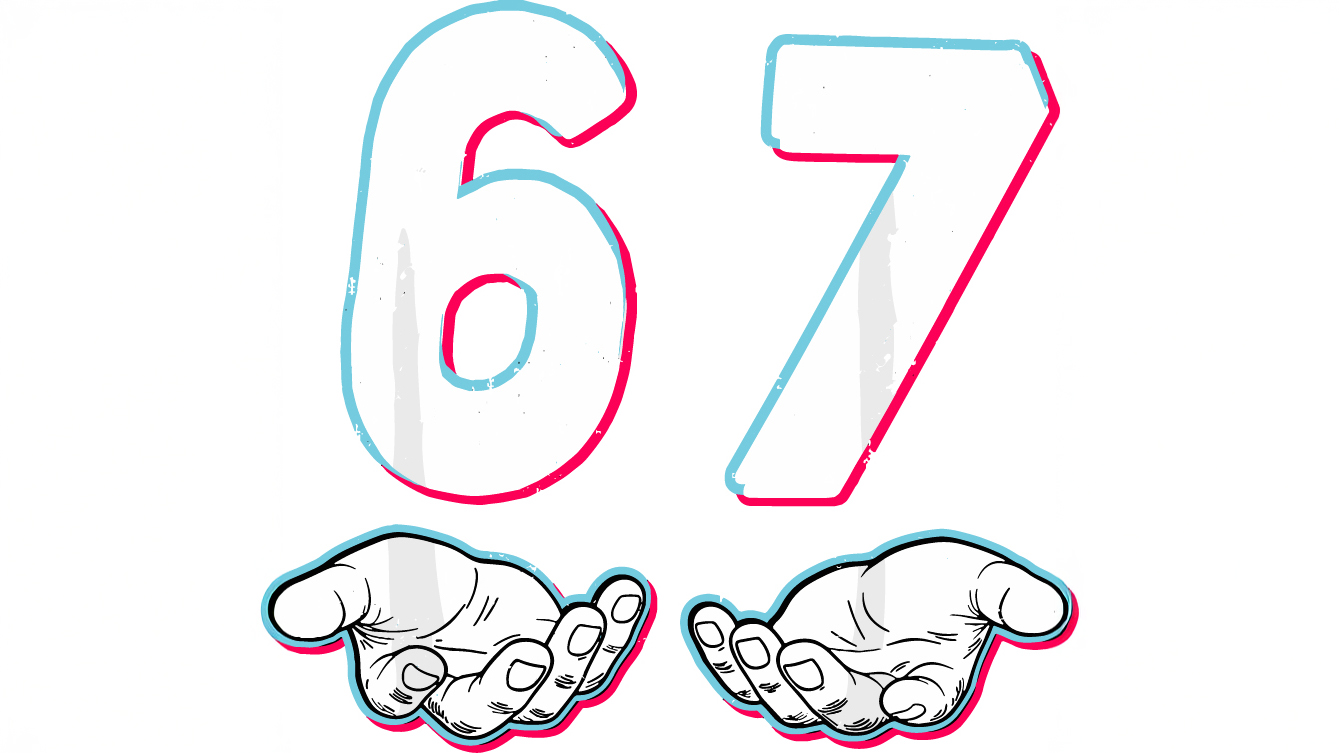
\includegraphics[width=0.8\textwidth]{images/67.jpg}
	    \caption{Problem Set 6-7... hehehe}
	    \label{fig:67}
	\end{figure}
	\vspace{1.25in}
	\begin{center}
	    \textit{Thank you, Mr. Kong}
	\end{center}
	\vfill
	\begin{center}
		{\large
		\textsc{Physica Vincit Omnia}
		}
	\end{center}
\end{document}
